% ------------------------------------------------------------------------------
% Chapter 1
% Delete this content and replace with your own
% ------------------------------------------------------------------------------
\chapter{Chapter Heading} % enter the name of the chapter here
\label{cha:chapter label} % enter the chapter label here (for cross referencing)

\blindtext[1] % Creates 
\blindtext[2] % Creates 

\section{Section Heading} % enter the name of the section here
\label{sec:section label} % enter the section label here (for cross referencing)

\blindtext[1]
 
\subsection{Subsection Heading} %enter the name of the subsection here
\label{sec:subsection label} % enter the subsection label here (for cross referencing)

\blindtext[1]

\subsection{Some maths}

% ------------------------------------------------------------------------------
% Math mode examples
% ------------------------------------------------------------------------------

\LaTeX\ is very good at presenting mathematics.

Inline equation :
$ax^2 + bx + c = 0$ % note use of single $ signs

Display equation:
$$x = \frac{-b \pm \sqrt{b^2 - 4ac}}{2a}$$ % note use of double $$ signs

Numbered equation:
\begin{align}
	\label{eq:equation label} % enter the equation label here (for cross referencing)
	\frac{\partial}{\partial t} U + \nabla \cdot F = 0
\end{align}

Aligned equation (not how equals signs line up):
\begin{align}
	\notag % means the current line will not be numbered
	\label{eq:dot product}
	\textbf{a} \cdot \textbf{b} &= \sum_{i=1}^n a_ib_i \\
	&= a_1b_1 + a_2b_2 + \cdots + a_nb_n; % the & is used as the alignment guide
\end{align}

Aligned equation with no numbers:
\begin{align*} % note use of *
	\label{eq:dot product}
	\textbf{a} \cdot \textbf{b} &= \sum_{i=1}^n a_ib_i \\
	&= a_1b_1 + a_2b_2 + \cdots + a_nb_n;
\end{align*}

\subsection{Theorems, proofs, definitions and examples}

% ------------------------------------------------------------------------------
% Theorems, proofs, definitions and examples
% ------------------------------------------------------------------------------
\begin{theorem}[Fermat's last theorem]
No three positive integers $a$, $b$, and $c$ satisfy the equation $a^n + b^n = c^n$ for any integer value of n greater than 2.
\end{theorem}

\begin{proof}
Left as an exercise for the reader.
\end{proof}

\begin{definition}
The intersection of two sets $A$ and $B$, denoted by $A \cap B$, is the set of all objects that are members of both the sets $A$ and $B$.
\end{definition}

\begin{example}
Given the two sets $A = \{x:x\in \mathbb{N}, x < 5\}$ and $B = \{x:x \in \mathbb{N}, x \text{ is even}\}$ then $A \cap B = \{2, 4\}$.
\end{example}


\section{Figures and tables}

% ------------------------------------------------------------------------------
% Figure example
% ------------------------------------------------------------------------------
\begin{figure}[H]
	\begin{center}
		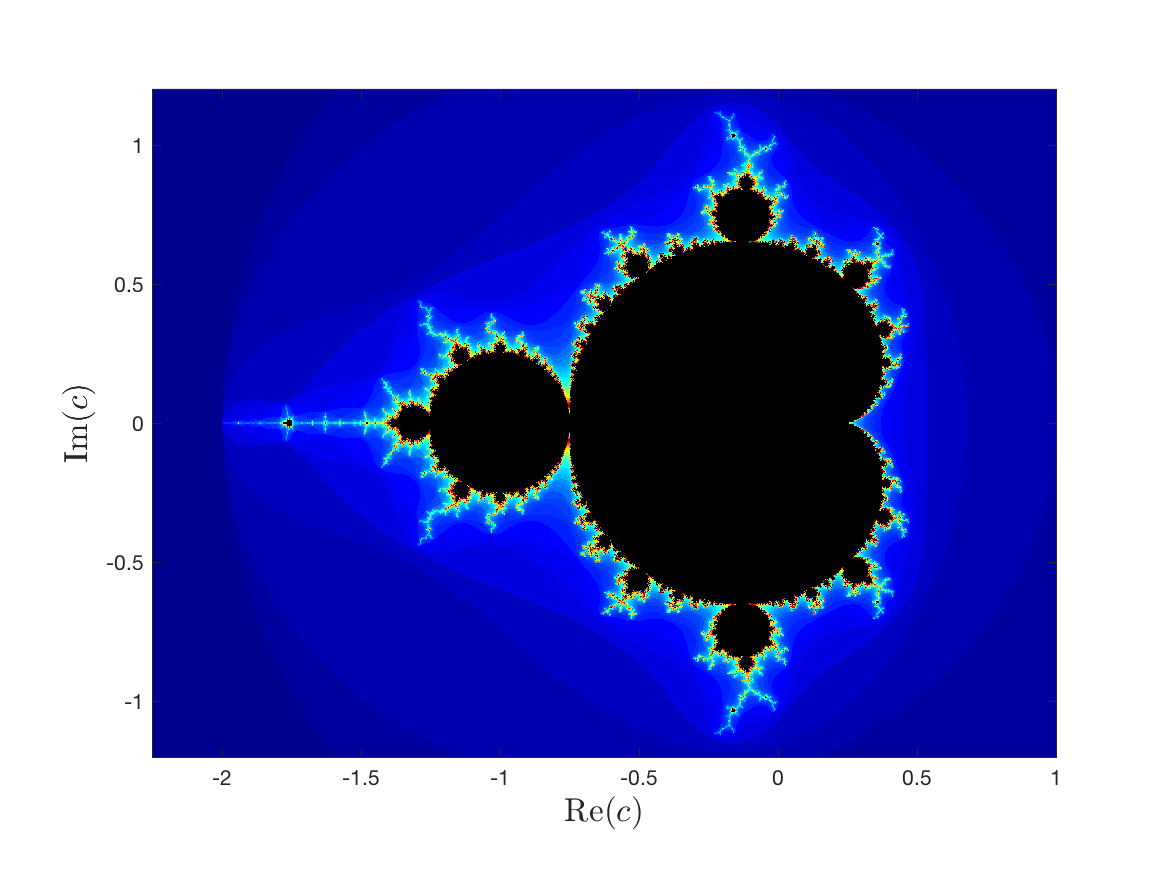
\includegraphics[width = 0.6\textwidth]{Images/mandelbrot} % enter the filename here
		\caption{This is a figure caption, note how it appears underneath the figure.} % enter the figure caption here
		\label{fig:figure label} % enter the figure label here (for cross referencing)
	\end{center}
\end{figure}

% ------------------------------------------------------------------------------
% Table example
% ------------------------------------------------------------------------------
\begin{table}[H]
	\caption{This is a table caption, not how it appears above the table.}
	\label{tab:table label} % enter the table label here (for cross referencing)
	\begin{center}
		\begin{tabular}{lcr} % three columns aligned left, centre and right respectively
			\toprule % thick horizontal line at the top of the table
			first column & second column & third column \\
			\midrule % single horizontal line separating the column headings
			This & This & This \\
			column & column & column \\
			is left & is centrally & is right \\
			aligned & aligned & aligned \\
			\bottomrule % thick horizontal line at the bottom of the table
		\end{tabular}
	\end{center}
\end{table}

\subsection{Program code}

% ------------------------------------------------------------------------------
% Code listing example
% ------------------------------------------------------------------------------
\begin{lstlisting}[style=matlabcode,
    caption = A MATLAB function to compute the first $n$ numbers of the Fibonacci series,
    label = mat:fibonacci
    ]
function y = fibonacci(n)

% This function calculates the first n terms in the Fibonacci series

y(1) = 0;
y(2) = 1;

for i = 3 : n
    y(i) = y(i-2) + y(i-1)
end

end
\end{lstlisting}

% ------------------------------------------------------------------------------
% Referencing examples
% ------------------------------------------------------------------------------
\section{Referencing}
References can be cited so that the author names(s) are a part of the sentence, e.g., \textcite{stroud:2013}, \textcite{harten:1983}

Alternatively, references can be cited so that the author names appear in the brackets (for when the name of the author is not relevant to the sentence), e.g., \parencite{stroud:2013},  \parencite{harten:1983}.

Cross referencing is easily done by using the label of the item you are referencing to (see source code for details).
\begin{itemize}
	\item Chapter~\ref{cha:chapter label}
	\item Section~\ref{sec:section label}
	\item Equation~(\ref{eq:equation label})
	\item Table~\ref{tab:table label}
	\item Figure~\ref{fig:figure label}
	\item Page~\pageref{eq:equation label}
\end{itemize}

Above is an example of a bulleted list. You can also create numbered lists:
\begin{enumerate}
	\item First list item
	\item Second list item
	\begin{enumerate}
		\item First sub list item
		\item Second sub list item
	\end{enumerate}
	\item Third list item
\end{enumerate}
